% mini eTPC parameter scans (2026-10-14 to 19, ELI-NP) — English version of scan_report_2026-10.tex (v4.3)
% build: lualatex scan_report_2026-10_en.tex (x2)
\documentclass[a4paper,11pt]{article}
\usepackage[top=22mm,bottom=22mm,left=20mm,right=20mm]{geometry}
\usepackage{fontspec}
\usepackage{graphicx}
\usepackage{booktabs}
\usepackage{array}
\usepackage{caption}
\usepackage{siunitx}
\usepackage{pgfplots}
\usetikzlibrary{calc}
\pgfplotsset{compat=1.18}
\usepackage{xcolor}
\usepackage[section]{placeins}
\usepackage{float}
\usepackage{url}
\urlstyle{tt}
\usepackage[colorlinks=true,linkcolor=blue!60!black,urlcolor=blue!60!black]{hyperref}
\captionsetup{font=small,labelfont=bf}
\sisetup{detect-all,range-phrase=--,range-units=single}
\setlength{\tabcolsep}{4pt}
\renewcommand{\arraystretch}{1.1}
\newcommand{\us}{\,\textmu s}
\newcommand{\uA}{\,\textmu A}

\title{mini eTPC parameter scans\\[2pt]
\large ELI-NP, 14--19 October 2026 (ELITPC DAQ, $\alpha$ source)}
\author{Soichiro Aogaki (compiled with Claude)}
\date{20 October 2026 --- informal working document for discussion\\
\small (English version of the Japanese report v4.3; runs 78--176)}

\begin{document}
\maketitle

\begin{abstract}
From 14 to 19 October 2026 we ran 19 parameter scans (runs 78--176, about 100 runs) on the ELI-NP mini eTPC
(GET electronics, one zCoBo, one AsAd = 272 channels), covering the electronics, the high voltage, the readout mode and the gas flow.
The six conclusions are:
(1) \textbf{Operating point B} --- GEM $240\,\mathrm{V} \times 3$, peaking time 502 ns $\times$ gain 120 fC, full readout, 25 MHz, triggerDelay 1750 --- is adopted for routine running (all metrics stable over a 9.6 h overnight run).
(2) The summed charge is fully collected for every peaking time; the peaking time only changes the peak height and the time width (shown by deconvolution).
(3) The gain follows $\ln G = \sum_i a_i \Delta V_i$ with $a \approx 0.014 \pm 0.0015$/V (the three foils agree within errors and the effects add up); up to $-30$ V in total on the GEMs can be compensated by the electronics.
(4) A single hit is measured to $\sigma_z \approx 0.20$ mm in drift direction (one time bin; constant in mm, independent of the HV and of the drift field) and to $\sigma \approx 0.30$ mm per view in the strip plane (232--502 ns).
(5) The rate limit is set by the zCoBo firmware readout time (2.94 ms for 272 channels, $\approx 340$ Hz; triggers arriving during readout are lost), not by the network. Zero suppression with per-channel thresholds (pedestal $+5\sigma$) reduces the data by 1/9--1/12 without any loss of quality; \textbf{the default candidate for beam runs is hit-register partial readout + ZS (23 kB/event)}.
(6) Halving the gas flow from 100 to 50 ml/min lowers the total charge by 3.5\,\%, settling within a few hours (the volume exchange time of the 54 L chamber); 150 and 200 ml/min give the same as 100 (the difference seen at 200 is a density change from a temperature rise of $\approx 1.3$ K). This is explained by the $S/Q$ term of the steady-state impurity concentration $c = c_\mathrm{bottle} + S/Q$; the HV is not involved.
\end{abstract}

\tableofcontents

\section{Setup and method}

\subsection{Apparatus and common conditions}
\begin{itemize}
\item Detector: mini eTPC (ELI-NP). 20 cm drift, triple GEM, U/V/W strip readout. CO$_2$ at 91 mbar.
\item Source: $^{228}$Th $\alpha$ source (outside the entrance wall, $x = -370$ mm). External trigger $\approx 4.6$ Hz.
\item Electronics: GET (4 AGET = 272 channels, 16 of them FPN), one zCoBo (firmware 2018-10-31), 25 MHz sampling (1 cell = 40 ns), 512 cells.
\item HV (CAEN DT1415ET, 8 channels in series, 200 M$\Omega$ resistor chain): ch0 TR1 (induction) 350 V, ch1/3/5 GEM1--3 (GEM1 = readout side), ch2/4 transfer 350 V, ch6/7 drift $600\,\mathrm{V} \times 2$.
  \textbf{GEMs at $250 \times 3$ for S1--S9 and at $240 \times 3$ from 15 Oct 12:50 (operating point B).}
\item DAQ: tpcdaq-rs (Rust) + root\_sink (C++) on the ELITPC host (repository in Appendix A). The electronics parameters are kept as JSON (template + knobs + exceptions); the settings and the HV of every run are logged automatically.
\item One scan point = one run (1,500 events $\approx$ 5.5 min unless stated otherwise).
\end{itemize}

\subsection{Definition of the metrics}
All metrics are computed per run by \texttt{tools/scan/run\_metrics.C}.
\begin{itemize}
\item Pedestal: mean of cells 1--20 of each channel (per-channel calibration table for ZS data); the mean FPN waveform is subtracted to remove common-mode noise. Hit threshold 35 ADC.
\item \textbf{Hit channels}: median number of channels above threshold. \textbf{Total charge}: median over events of the sum of all samples.
\item \textbf{Saturation}: fraction of events with a channel at 4095 ADC. \textbf{Clip}: fraction of events whose band touches the start or end of the time window.
\item \textbf{ok / length / dEdx}: result of fitting one straight line per event with the analysis macros (\texttt{analyzeUVW.C} + \texttt{makeTracks.C}, S.~Aogaki). ok = fraction of successful fits, length = median track length [mm], dEdx = median / IQR of the charge per unit length (ADC/mm).
\item $\sigma_z$: robust $\sigma$ of the hit z residuals with respect to the line (\texttt{hit\_residuals.C}). $\sigma_{2D}$: robust $\sigma$ of the U+V+W closure residual divided by $\sqrt{3}$ (\texttt{uvw\_closure.C}, Sec.~\ref{sec:closure}).
\end{itemize}

\subsection{Terms and abbreviations}
\begin{description}
\item[GET / AGET / AsAd / zCoBo] GET = General Electronics for TPCs. AGET = ASIC with 64 signal + 4 FPN channels (preamplifier, shaper, switched-capacitor array). AsAd = board carrying 4 AGETs (272 channels). zCoBo = Zynq (ZC706) board that reads the AsAd and sends the data to the PC, and its firmware (FW).
\item[FPN] Fixed Pattern Noise channels: the 4 of the 68 AGET channels that are not connected to the detector (ch 11, 22, 45, 56). They carry only the noise common to the signal path, so their mean waveform is subtracted from the signals to remove common-mode noise.
\item[cell / bucket] One SCA sample. At 25 MHz one cell = 40 ns; one event = 512 cells.
\item[peaking time / gain] AGET shaper peaking time (70 / 232 / 502 / 1014 ns) and preamplifier full-scale charge (120 fC / 240 fC / 1 pC). A larger gain value means a lower amplification.
\item[full / partial readout, hit register] Full = read all channels. Partial = read only the channels flagged in the AGET hit register (above threshold). With \texttt{channel Reading = always}, partial readout still reads all channels.
\item[frameType 1 / 2] zCoBo output formats. 1 = 4 B/sample with channel number (partial, ZS); 2 = compact 2 B/sample (full readout only).
\item[ZS] Zero suppression: the zCoBo FW does not send samples below a per-channel threshold.
\item[ped] Pedestal (ADC value without signal, $\approx 450$ ADC per channel).
\item[IQR] Interquartile range (75\,\% minus 25\,\% quantile); a width that is robust against outliers.
\item[robust $\sigma$] $1.4826 \times$ MAD (median absolute deviation). Equal to $\sigma$ for a Gaussian, not pulled by heavy tails.
\item[FWHM] Full width at half maximum. \textbf{S/N}: signal-to-noise ratio. \textbf{GEM}: Gas Electron Multiplier, three foils here. \textbf{TR}: transfer gap between GEMs; \textbf{TR1}: induction gap between GEM1 and the readout plane.
\item[U / V / W, view] The three strip families of the readout plane (inclined by 60$^\circ$ to each other). ``One view'' = the one-dimensional image seen by one strip family.
\end{description}

\subsection{List of scans}
\begin{table}[H]\centering\small
\caption{Scan index (S numbers as in the scan ledger \texttt{docs/SCANS\_ja.md}).}
\begin{tabular}{llllp{70mm}}
\toprule
\# & Date & Scan & Runs & Conclusion \\
\midrule
S1 & 10-14 & triggerDelay, 5 points & 78--82 & Band position linear, $508 - \mathrm{delay}/4$; set to 1750 \\
S2 & 10-14 & peaking time, 4 points & 83--86 & 70 ns loses tracks, 1014 ns saturates in 1/3 of events \\
S3 & 10-14 & gain, 4+1 points & 87--90, 112 & E rule gives 502 ns $\times$ 240 fC; 1 pC unusable \\
S4 & 10-14 & pulser response kernel, 8 points & 102--110 & Kernel has no ringing; $\alpha$ ``wiggle'' is not from the electronics \\
S5 & 10-14 & pedestal, 2 points & 99, 100 & Per-channel tables (232 / 502 ns) \\
S6 & 10-14 & drift end at 12.5 MHz & 111, 113 & Source position too far out to span z; retry with the source inside \\
S7 & 10-14/15 & overnight $\alpha$ run (E) & 114 & Stable over 10 h, 166k events \\
S8 & 10-14 & deconvolution & 84--88 & Sum of samples collects all charge at any peaking time \\
S9 & 10-15 & readout / hit threshold / ZS & 115--121 & Old partial mode read all channels: twice the data of full \\
S10 & 10-15 & GEM voltage margin & 122--129 & $\ln G \approx 0.014$/V $\times \Delta V$, tracks intact down to $-30$ V \\
S11 & 10-15 & hit z residual & (analysis) & $\sigma_z \approx 0.2$ mm = 1 cell \\
S12 & 10-15 & drift voltage, 3 points & 130--132 & $v \propto E$; $\sigma_z$ constant in mm \\
S13 & 10-15 & ZS, per-channel threshold & 133 & 31.8 kB/event (1/8.8); macros need an update \\
S14 & 10-15 & U/V/W closure residual & (analysis) & $\sigma_{2D} = 0.30$ mm/view \\
S15 & 10-15 & hit-register threshold, 6 points & 135--140 & Threshold works, but at most 14\,\% below full \\
S16 & 10-15/16 & overnight $\alpha$ run (B) & 141 & Stable over 9.6 h; B adopted \\
S17 & 10-16 & maximum rate & 148--169 & Limit = FW readout time 2.94 ms \\
S18 & 10-16 & ZS validation & 170--173 & No quality loss, 1/9--1/12 of the data; suppress FPN \\
S19 & 10-16/21 & gas flow, 4 points & 174--178 & $-3.5$\,\% charge at 50, settles in hours; 150 and 200 same as 100 (the 200 difference is temperature) \\
\bottomrule
\end{tabular}
\end{table}

\section{Electronics parameters}

\subsection{triggerDelay (S1)}
25 MHz, 232 ns, 120 fC, partial readout. The first cell of the band (median first hit) is strictly linear in the delay,
$\mathrm{first} = 508 - \mathrm{delay}/4$ (delay in units of 10 ns). At a delay of 2000, 15\,\% of the events are cut at the start and ok drops to 0.86.
The setting was changed from 1500 to \textbf{1750} (band starts $\approx 2.8$\us before the trigger). Rule: $\mathrm{delay}\,[10\,\mathrm{ns}] = (\text{window}\,[\mathrm{ns}] - 2800 - 160)/10$ (1750 at 25 MHz, 3800 at 12.5 MHz).

\begin{figure}[h]\centering
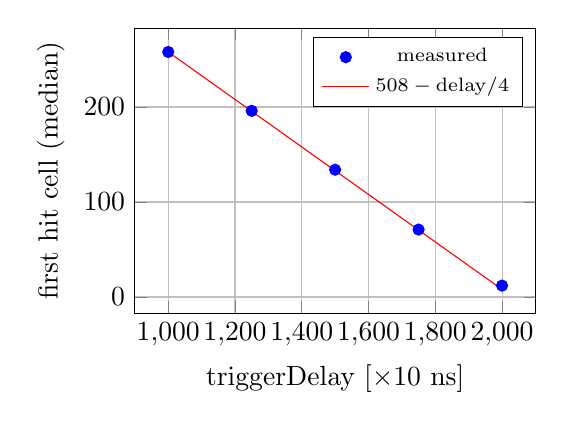
\begin{tikzpicture}
\begin{axis}[width=0.55\textwidth,height=5.2cm,xlabel={triggerDelay [$\times$10 ns]},ylabel={first hit cell (median)},grid=major,legend pos=north east,legend style={font=\scriptsize}]
\addplot[only marks,mark=*,blue] coordinates {(1000,258)(1250,196)(1500,134)(1750,71)(2000,12)};
\addlegendentry{measured}
\addplot[red,domain=1000:2000,samples=2] {508 - x/4};
\addlegendentry{$508 - \mathrm{delay}/4$}
\end{axis}
\end{tikzpicture}
\caption{S1: first cell of the band versus triggerDelay (runs 78--82).}
\end{figure}

\begin{table}[h]\centering\small
\caption{S1 triggerDelay (runs 78--82).}
\begin{tabular}{rrrrrrrr}
\toprule
delay & run & first (p10--p90) & last (p90) & clip at start & hit ch & ok & length [mm] \\
\midrule
1000 & 78 & 258 (243--264) & 282 (325) & 0 & 121 & 0.997 & 84.4 \\
1250 & 79 & 196 (182--201) & 220 (263) & 0 & 121 & 0.998 & 84.4 \\
1500 & 80 & 134 (119--139) & 157 (198) & 0 & 119 & 0.993 & 83.9 \\
1750 & 81 & 71 (55--76) & 94 (142) & 0.001 & 120 & 0.992 & 84.1 \\
2000 & 82 & 12 (3--16) & 31 (74) & \textbf{0.154} & 75 & \textbf{0.863} & \textbf{68.1} \\
\bottomrule
\end{tabular}
\end{table}

\subsection{Peaking time (S2), response kernel (S4) and deconvolution (S8)}
Delay 1750, 120 fC, GEMs at $250 \times 3$. Longer shaping picks up weaker strips (hit channels $121 \to 147$) but saturates more: at 1014 ns one third of the events saturate.
At 70 ns the S/N is too low and one third of the tracks is lost.

\begin{table}[h]\centering\small
\caption{S2 peaking time (runs 83--86).}
\footnotesize
\begin{tabular}{rrrrrrrrrr}
\toprule
peaking & run & width [cell] & hit ch & total charge & sat. & ok & length / IQR & dEdx / IQR & wiggle A0 [ADC] \\
\midrule
70 ns & 83 & 25 & 52 & 0.25 M & 0.0\,\% & 0.660 & 45.4 / 46.3 & 4,602 / 855 & 4.4 \\
232 ns & 84 & 39 & 121 & 1.40 M & 0.3\,\% & 0.998 & 85.2 / 58.4 & 12,493 / 6,438 & 12.4 \\
502 ns & 85 & 62 & 128 & 3.24 M & 4.8\,\% & 0.997 & 88.9 / 58.8 & 19,087 / 9,466 & 27.9 \\
1014 ns & 86 & 106 & 147 & 7.21 M & 33.7\,\% & 0.998 & 104.5 / 66.6 & 22,469 / 9,693 & 59.9 \\
\bottomrule
\end{tabular}
\end{table}

The total charge grows as 1 : 2.3 : 5.2 with the peaking time. We first read this as ``short shaping integrates only part of the signal''; that was \textbf{wrong} --- it is an area effect (S8).
The \textbf{pulser response kernel} is the impulse response of the electronics (preamplifier + shaper + SCA). The AsAd has a built-in pulser that injects the same known charge (a voltage step of $-300$ / $-100$ mV on the test capacitor) into the test inputs of all AGET channels at once. The injected pulse is much shorter than a detector signal (effectively a $\delta$ function), so the kernel is obtained by aligning the output waveforms of all channels at their peak, averaging and normalising to the peak (one run averages $68 \times 4 \times 600 \approx 150{,}000$ waveforms, Fig.~\ref{fig:kernel}). A detector waveform is ``arrival-time distribution of the charge $\otimes$ kernel'', so knowing the kernel one can deconvolve back to the arrival-time distribution (S8). The measured kernels are identical for the four AGETs and show no ringing (1.8\us component $\le 0.03$\,\%); the peak gain ratio is 232 : 502 : 1014 = 1 : 1.05 : 1.17.
Deconvolving the $\alpha$ waveforms with these kernels (\texttt{deconv.C}, FFTW, $\lambda_\mathrm{rel} = 10^{-3}$) brings the charge ratio back to 1 : 1.05 : 1.21, matching the pulser gain ratio.
In other words, \textbf{the sum of samples collects the full input charge at every peaking time}. After deconvolution the FWHM converges to 13.7 / 14.6 / 18.7 cells (0.55--0.75\us), the intrinsic width on the detector side (Fig.~\ref{fig:deconv}).
Because of the noise amplification (S/N $\times$ 0.4--0.5) we do not use it online; it stays as an offline option ($\lambda = 10^{-2}$).

The ``wiggle'' with a period of 1.6--1.8\us seen on $\alpha$ waveforms (signal channels only, proportional to the charge) is absent from the kernel, so it is not a response of the AGET shaping (origin unknown, Sec.~\ref{sec:open}).

\begin{figure}[h]\centering
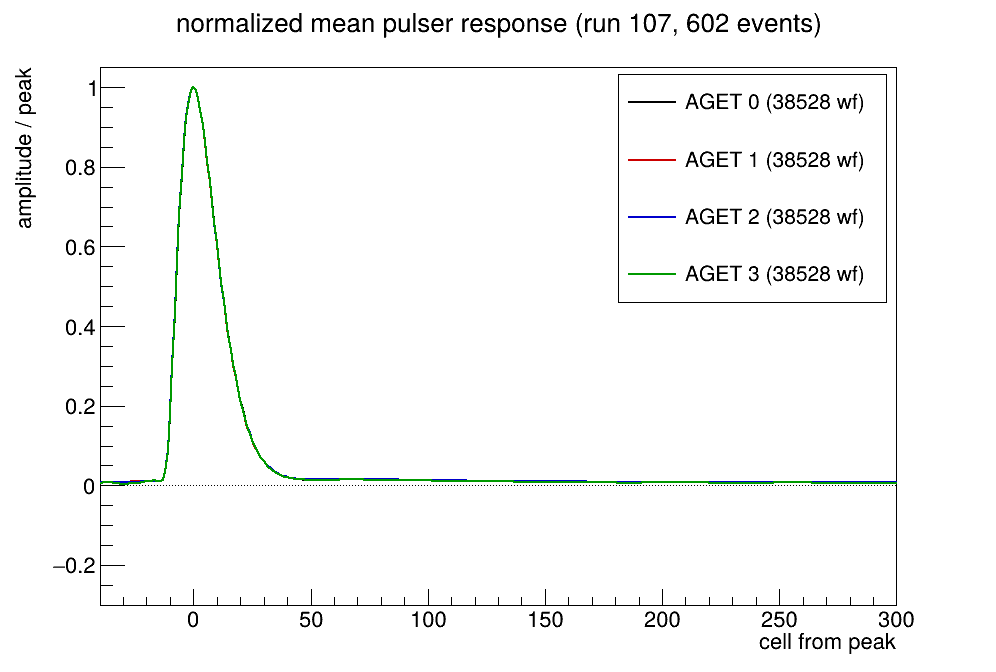
\includegraphics[width=0.48\textwidth]{fig/kernel2/run0107_kernel.png}\hfill
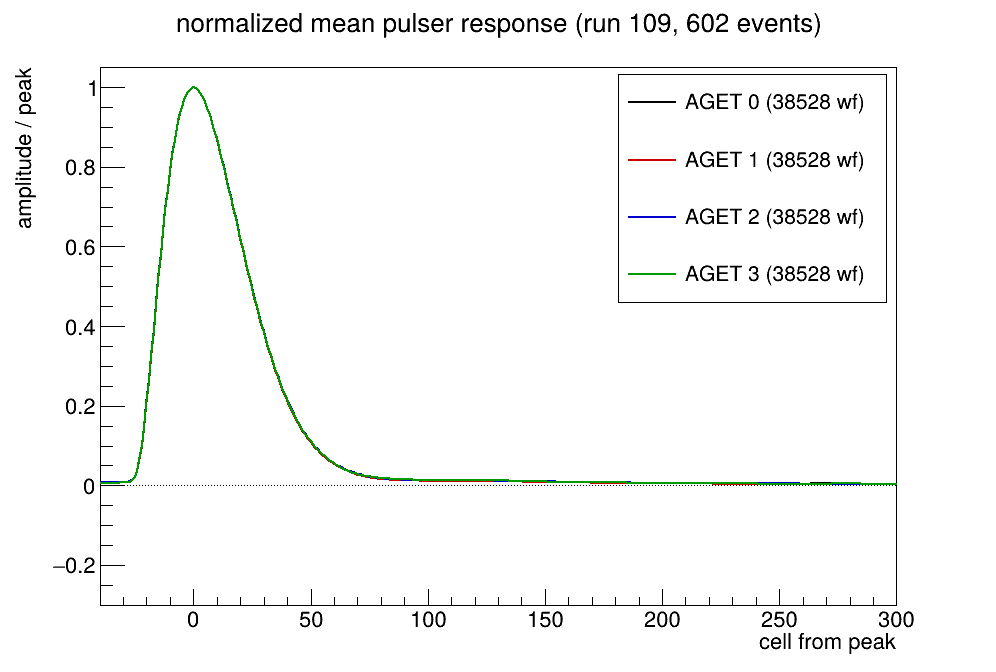
\includegraphics[width=0.48\textwidth]{fig/kernel2/run0109_kernel.png}
\caption{S4: pulser response kernels (left: 502 ns, run 107; right: 1014 ns, run 109). Mean waveform of each AGET normalised to the peak. No ringing.}
\label{fig:kernel}
\end{figure}

\begin{figure}[h]\centering
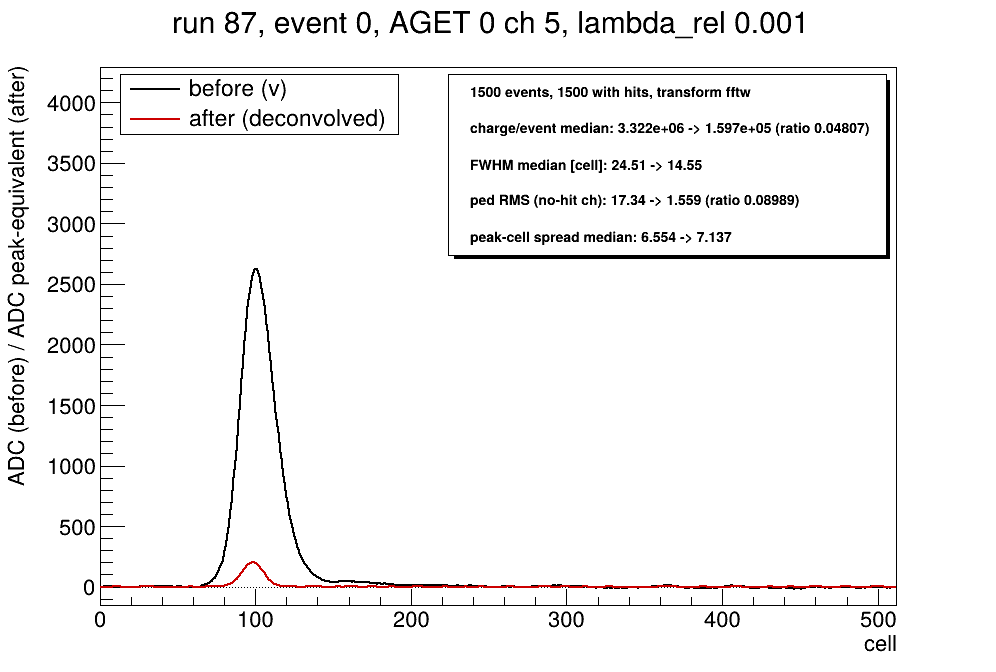
\includegraphics[width=0.6\textwidth]{fig/deconv/run0087_k107_l1e-3.png}
\caption{S8: one channel of run 87 (502 ns $\times$ 120 fC) before and after deconvolution. FWHM $24.5 \to 14.6$ cells; charge ratio 0.048 (normalised by the kernel sum).}
\label{fig:deconv}
\end{figure}

\subsection{Gain (S3) and the E rule}
502 ns, GEMs at $250 \times 3$. The ``E rule'' --- take the longest peaking time, with its gain, that keeps the fraction of events with a saturated channel below 2\,\% --- selects \textbf{502 ns $\times$ 240 fC} (0.7\,\% saturation) at $250 \times 3$.
At 1 pC the tracks fall below the 35 ADC threshold (ok 0.009). The wiggle amplitude scales with the output amplitude (it rides on the gain).

\begin{table}[h]\centering\small
\caption{S3 gain (runs 87--90, 112).}
\begin{tabular}{lrrrrrrrr}
\toprule
peaking $\times$ gain & run & hit ch & total charge & sat. & clip start/end & ok & length / IQR & dEdx / IQR \\
\midrule
502 $\times$ 120 fC & 87 & 127 & 3.20 M & 4.7\,\% & 8.3 / 21.4\,\% & 0.997 & 88.2 / 58.8 & 19,352 / 9,283 \\
\textbf{502 $\times$ 240 fC} & 88 & 119 & 1.71 M & \textbf{0.7\,\%} & 2.7 / 8.9\,\% & 0.991 & 84.0 / 59.3 & 11,946 / 5,896 \\
502 $\times$ 1 pC & 89 & 23 & 0.16 M & 0\,\% & 0 / 0.1\,\% & 0.009 & --- & --- \\
1014 $\times$ 1 pC & 90 & 43 & 0.53 M & 0\,\% & 0 / 0.1\,\% & 0.626 & 48.3 / 50.2 & 3,669 / 820 \\
1014 $\times$ 240 fC & 112 & 122 & 3.90 M & 2.1\,\% & 0.7 / 4.8\,\% & 0.998 & 84.6 / 58.4 & 16,155 / 7,814 \\
\bottomrule
\end{tabular}
\end{table}

\section{Detector high voltage and gas}

\subsection{GEM voltage margin (S10)}
On site, the GEMs were lowered one at a time or all three together (HV set by hand with CAEN GECO, runs with \texttt{gem\_point.sh}), and the total charge was compared with the same electronics (502 ns $\times$ 120 fC).
As Fig.~\ref{fig:gain} shows, $\ln(Q/Q_0)$ is explained by the sum of the $\Delta V$ of the three foils. The individual slopes GEM1 / GEM2 / GEM3 = 0.0148 / 0.0130 / 0.0145 $\pm$ 0.0026/V agree within errors,
and the sum of the three single-foil points ($-0.423 \pm 0.045$) equals the all-three point ($-0.425 \pm 0.026$), so the effects add. Mean slope $a = 0.0141 \pm 0.0015$/V (a factor 0.86 per $-10$ V in total).
Down to $-30$ V in total ($240$ V each, the same value as the full-size HIGS detector), the electronics compensate and the track quality (ok, hit channels, length, relative dEdx width) does not change; no trips or current anomalies occurred.
The currents are about 8.6--8.8\uA on all channels and follow the voltage ratio when the GEMs are lowered. The 200 M$\Omega$ resistor chain on the HV side, as Traian explained earlier from the circuit diagram, is also clearly confirmed by the present V--I data: the summed voltage of ch0--5, 1,770 V at $240 \times 3$, divided by 200 M$\Omega$ gives 8.85\uA against a measured 8.63--8.80\uA; at $250 \times 3$, 1,800 V gives 9.0\uA against 8.80\uA.

\begin{figure}[H]\centering
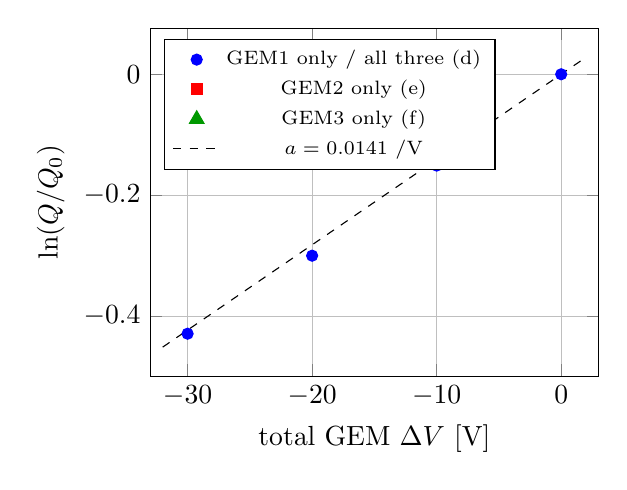
\begin{tikzpicture}
\begin{axis}[width=0.6\textwidth,height=6cm,xlabel={total GEM $\Delta V$ [V]},ylabel={$\ln(Q/Q_0)$},grid=major,legend pos=north west,legend style={font=\scriptsize},xmin=-33,xmax=3]
\addplot[only marks,mark=*,blue] coordinates {(0,0)(-10,-0.151)(-20,-0.300)(-30,-0.429)};
\addlegendentry{GEM1 only / all three (d)}
\addplot[only marks,mark=square*,red] coordinates {(-10,-0.130)};
\addlegendentry{GEM2 only (e)}
\addplot[only marks,mark=triangle*,green!60!black,mark size=3pt] coordinates {(-10,-0.145)};
\addlegendentry{GEM3 only (f)}
\addplot[black,dashed,domain=-32:2,samples=2] {0.0141*x};
\addlegendentry{$a = 0.0141$ /V}
\end{axis}
\end{tikzpicture}
\caption{S10: gain law. Each point has an error of $\pm 0.026$ (median charge of 1,500 events).}
\label{fig:gain}
\end{figure}

\begin{table}[H]\centering\small
\caption{S10 GEM voltages (compared at 502 ns $\times$ 120 fC; point a = reference run 87).}
\footnotesize
\begin{tabular}{llrrrrrrr}
\toprule
point & GEM1 / GEM2 / GEM3 [V] & run & hit ch & total charge & sat. & ok & length & dEdx / IQR \\
\midrule
a & 250 / 250 / 250 & 87 & 127 & 3.20 M & 4.7\,\% & 0.997 & 88.2 & 19,352 / 9,283 \\
b & 240 / 250 / 250 & 122 & 124 & 2.76 M & 2.6\,\% & 0.999 & 85.9 & 17,645 / 8,645 \\
c & 230 / 250 / 250 & 123 & 122 & 2.38 M & 1.1\,\% & 0.997 & 84.7 & 15,258 / 7,697 \\
d & 240 / 240 / 240 & 126 & 121 & 2.09 M & 1.0\,\% & 1.000 & 84.3 & 13,637 / 6,617 \\
e & 250 / 240 / 250 & 128 & 125 & 2.81 M & 2.0\,\% & 0.996 & 86.3 & 17,553 / 8,318 \\
f & 250 / 250 / 240 & 129 & 123 & 2.76 M & 2.3\,\% & 0.999 & 84.9 & 17,726 / 8,566 \\
\bottomrule
\end{tabular}
\end{table}

\subsection{Drift voltage (S12)}
At operating point B the drift voltage was set to 1,000 / 1,200 / 1,400 V ($500 / 600 / 700\,\mathrm{V} \times 2$). The time width of the band times V is constant ($\pm 6$\,\%), so $v_\mathrm{drift} \propto E$, consistent with the nominal $v = 0.7233 \times E/p$.
The pulse width goes $61 \to 57 \to 54$ cells ($-11$\,\% for $+40$\,\% in E: the $1/\sqrt{E}$ of diffusion plus the shaping width). Total charge and hit channels do not change (no loss in focusing into GEM3).
$\sigma_z$ scales as $1/v$ in cells but is \textbf{constant in mm (0.207 / 0.208 / 0.208)}. Routine running stays at 1,200 V.

\begin{table}[H]\centering\small
\caption{S12 drift voltage (runs 130--132, operating point B).}
\begin{tabular}{rrrrrrrrr}
\toprule
$V_\mathrm{drift}$ & run & time width [cell] & width $\times$ V & pulse width [cell] & hit ch & total charge & $\sigma_z$ [cell] & $\sigma_z$ [mm] \\
\midrule
1,000 & 131 & 28 & 28,000 & 61 & 120 & 2.07 M & 1.30 & 0.207 \\
1,200 & 130 & 22 & 26,400 & 57 & 121.5 & 2.09 M & 1.09 & 0.208 \\
1,400 & 132 & 20 & 28,000 & 54 & 123 & 2.09 M & 0.93 & 0.208 \\
\bottomrule
\end{tabular}
\end{table}

\subsection{Operating point B and overnight runs (S7, S16)}
\textbf{Operating point B} (GEM $240 \times 3$, 502 ns $\times$ 120 fC, full readout, 25 MHz, delay 1750, drift $600 \times 2$, transfer 350) was adopted on 15 October at 12:50.
The GEMs run 10 V per foil lower, and full readout uses frameType 2 (2 B/sample), so the data size is half of that of setting A (partial, 557 kB/event): 278.8 kB/event.
The metrics of the overnight run 141 (9.6 h, 149,795 events, 4.32 Hz, 104 GB) agree with the 5.5 min check run 130 and with the overnight run of setting A (run 114, 10 h, 166,386 events).

\begin{table}[H]\centering\small
\caption{Overnight runs (S7, S16).}
\scriptsize\setlength{\tabcolsep}{3pt}
\begin{tabular}{llrrrrrrrrr}
\toprule
run & setting & events & kB/ev & hit ch & charge & sat. & ok & length / IQR & $\sigma_z$ & $\sigma_{2D}$ \\
\midrule
114 & A overnight ($250{\times}3$, 502${\times}$240 fC, partial) & 166,386 & 557 & 119 & 1.71 M & 0.62\,\% & 0.995 & 83.4 / 59.6 & 0.20 & 0.325 \\
130 & B check (5.5 min) & 1,500 & 278.8 & 121.5 & 2.09 M & 0.60\,\% & 0.998 & 84.4 / 58.5 & 0.21 & 0.314 \\
\textbf{141} & \textbf{B overnight} & 149,795 & 278.8 & 121 & 2.08 M & 0.92\,\% & 0.999 & 84.1 / 58.8 & 0.20 & 0.321 \\
\bottomrule
\end{tabular}
\end{table}

\subsection{Gas flow (S19)}
Keeping operating point B, only the CO$_2$ flow was changed, 100 $\to$ 50 $\to$ 150 $\to$ 200 ml/min (54 L chamber, 91 mbar; run 174 at 100, run 175 at 50 for 67.7 h, run 176 at 150, run 178 at 200 for 17.2 h).
\texttt{gas\_trend.C} splits the raw tree into 1 h (run 175) or 10 min (runs 174, 176) bins and follows the median event charge and other quantities (Fig.~\ref{fig:gas}).

\begin{table}[H]\centering\small
\caption{S19 gas flow (whole-run metrics; run 176 includes the first 1.5 h of rise, its equilibrium value is 2.087 M).}
\begin{tabular}{rlrrrrrrr}
\toprule
run & flow & events & hit ch & charge & sat. & ok & length / IQR & dEdx / IQR \\
\midrule
174 & 100 ml/min & 11,145 & 120 & 2.077 M & 1.0\,\% & 0.999 & 84.1 / 58.9 & 13,532 / 6,508 \\
175 & 50 ml/min (67.7 h) & 1,057,719 & 120 & \textbf{2.002 M} & 0.9\,\% & 0.999 & 83.8 / 58.9 & 12,998 / 6,336 \\
176 & 150 ml/min (4.7 h) & 73,652 & 121 & 2.078 M & 1.0\,\% & 0.997 & 84.2 / 58.7 & 13,493 / 6,539 \\
178 & 200 ml/min (17.2 h) & 265,185 & 124 & 2.106 M & 0.9\,\% & 0.999 & \textbf{86.3} / 56.8 & 13,929 / 6,621 \\
\bottomrule
\end{tabular}
\end{table}

\begin{figure}[tbp]\centering
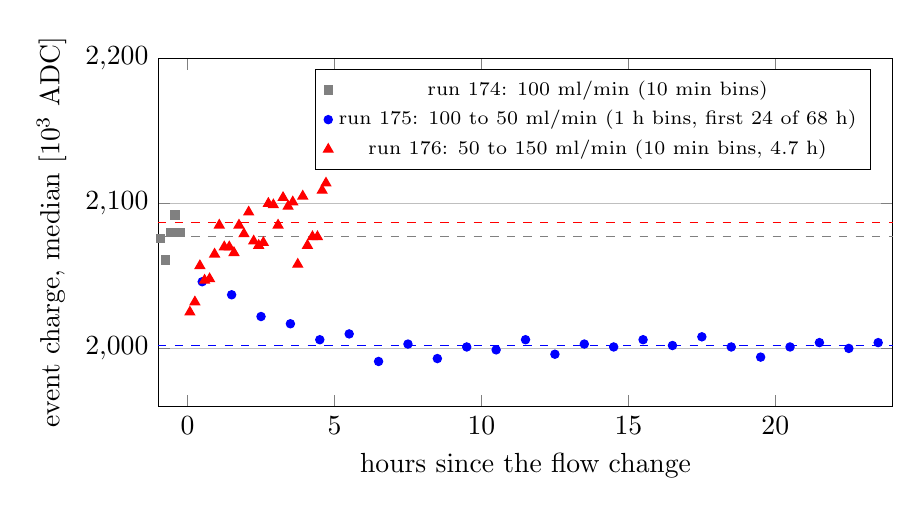
\begin{tikzpicture}
\begin{axis}[width=0.9\textwidth,height=6cm,xlabel={hours since the flow change},ylabel={event charge, median [$10^3$ ADC]},ymin=1960,ymax=2200,xmin=-1,xmax=24,ymajorgrids=true,legend pos=north east,legend style={font=\scriptsize}]
\addplot[only marks,mark=square*,gray,mark size=1.5pt] coordinates {(-0.92,2076) (-0.75,2061) (-0.58,2080) (-0.42,2092) (-0.25,2080)};
\addlegendentry{run 174: 100 ml/min (10 min bins)}
\addplot[only marks,mark=*,blue,mark size=1.5pt] coordinates {(0.50,2046) (1.50,2037) (2.50,2022) (3.50,2017) (4.50,2006) (5.50,2010) (6.50,1991) (7.50,2003) (8.50,1993) (9.50,2001) (10.50,1999) (11.50,2006) (12.50,1996) (13.50,2003) (14.50,2001) (15.50,2006) (16.50,2002) (17.50,2008) (18.50,2001) (19.50,1994) (20.50,2001) (21.50,2004) (22.50,2000) (23.50,2004)};
\addlegendentry{run 175: 100 to 50 ml/min (1 h bins, first 24 of 68 h)}
\addplot[only marks,mark=triangle*,red,mark size=2pt] coordinates {(0.08,2025) (0.25,2032) (0.42,2057) (0.58,2047) (0.75,2048) (0.92,2065) (1.08,2085) (1.25,2070) (1.42,2070) (1.58,2066) (1.75,2085) (1.92,2079) (2.08,2094) (2.25,2074) (2.42,2071) (2.58,2073) (2.75,2100) (2.92,2099) (3.08,2085) (3.25,2104) (3.42,2098) (3.58,2101) (3.75,2058) (3.92,2105) (4.08,2071) (4.25,2077) (4.42,2077) (4.58,2109) (4.71,2114)};
\addlegendentry{run 176: 50 to 150 ml/min (10 min bins, 4.7 h)}
\addplot[gray,dashed,forget plot,domain=-1:24,samples=2] {2077};
\addplot[blue,dashed,forget plot,domain=-1:24,samples=2] {2002};
\addplot[red,dashed,forget plot,domain=-1:24,samples=2] {2087};
\end{axis}
\end{tikzpicture}
\caption{S19: total charge after each flow change. Dashed lines: equilibrium value for each flow (grey 100 ml/min 2.077 M, blue 50 ml/min 2.002 M, red 150 ml/min 2.087 M). Statistical precision $\pm 0.5$\,\% per 1 h bin, $\pm 1$\,\% per 10 min bin. Run 175 stays flat at $2.00 \pm 0.01$ M from 24 h to 68 h (no day--night cycle). Run 176 ended at 4.7 h on an external HV interlock (from the gas system; no precursor in voltages or currents).}
\label{fig:gas}
\end{figure}

\begin{itemize}
\item At 50 ml/min the total charge drops from 2.08 to 2.00 M ($-3.5$\,\%) and dEdx by $-4$\,\%. The 16\,\% quantile drops by the same ratio: the whole distribution shrinks uniformly. Hit channels, track length, ok, band position (first 75 / last 98 cells) and pulse width (56 cells) are unchanged, so the drift velocity and diffusion are unchanged. The HV (1 h means from InfluxDB, 69 points) stayed within $\pm 0.05$ V and $\pm 0.5$\,\% in current: not involved.
\item The new equilibrium is reached within a few hours, and the rise after returning to 150 ml/min takes about 0.5 h. This matches the time constant for flushing 54 L at the given flow (at 91 mbar the actual volume flow is 11 times the normal flow: 1.6 h at 50 ml/min, 0.54 h at 150 ml/min); no slow process such as wall outgassing is needed.
\item Interpretation: the steady-state impurity concentration (mainly H$_2$O and air from leaks) is $c = c_\mathrm{bottle} + S/Q$ ($S$ = production inside the system, $Q$ = flow). The bottle term does not depend on the flow and drops out of the difference. The values 2.002 / 2.077 / 2.087 $\pm$ 0.004 M at 50 / 100 / 150 ml/min (150: mean of twenty 10 min bins between 1.5 and 4.7 h) are consistent within 1\,\% with a dependence on $S/Q$; above 100 ml/min the gain hardly changes. Practical consequences: \textbf{do not let a calibration span the few hours after a flow change}, and record the flow as part of the calibration conditions.
\item \textbf{The difference in run 178 (200 ml/min) is temperature, not flow.} The charge is flat for 17 h at 2.106 M ($+0.9$\,\% over 150), but the 16\,\% quantile rises by 6\,\%, hit channels by 3 and the track length by 2.5\,\%: not a uniform gain change. All three stopping $\alpha$ lines stop 1.5--1.9 mm further in ($^{224}$Ra 25.5 $\to$ 27.0, $^{212}$Bi 43.7 $\to$ 45.5, $^{220}$Rn 85.5 $\to$ 87.2 mm); relative to the full range including the 315 mm dead path, all three give the same \textbf{density change of $-0.45$\,\%}. Crossing tracks keep their length and gain 1.4\,\% in charge, so the gain is up by $\approx 2$\,\%. A $-0.45$\,\% density change corresponds to $+1.3$ K, consistent with the experimental area having been open during the day (more water in the gas would lower the gain instead). \textbf{The gain changes by $\approx 1.5$\,\%/K}, the same size as the flow effect, so comparisons need temperature and pressure records. The stopping positions of the $\alpha$ lines act as a densitometer and separate density from gain (applied to run 175, most of its $-3.5$\,\% remains a flow effect).
\item By-product: in the length $\times$ charge plane the $\alpha$ lines of the $^{228}$Th chain separate ($^{220}$Rn 6.29 MeV stops at 85 mm, $^{212}$Bi at 45 mm, $^{224}$Ra at 25 mm; $^{216}$Po and $^{212}$Po cross the active volume at 105 mm). Because the source sits 315 mm outside, the charge FWHM of the stopping lines is poor (19--31\,\%). This is the starting point for the metrics of the coming pressure scan.
\end{itemize}

\section{Hit precision}

\subsection{Definition of hits and of the two residuals}\label{sec:residual-def}
So that this section can be followed without doing track reconstruction, ``precision'' is defined in three steps.

\paragraph{1. Hit (one strip = one point).}
The analysis macro \texttt{analyzeUVW.C} makes exactly one point from the waveform of each strip channel (after pedestal subtraction).
It takes the samples above threshold (35 ADC) within $\pm 5$ cells of the maximum cell $t_\mathrm{peak}$ and computes
the charge $q = \sum v_t$ and the time $\bar t = \sum v_t\, t / q$ (charge-weighted).
Then $z = \bar t \times 40\,\mathrm{ns} \times v_\mathrm{drift}$ (1 cell = 0.19 mm), and the strip position $s$ [mm] comes from the channel map.
A hit is therefore (view, $s$, $z$, $q$): a two-dimensional point ``strip position $\times$ drift direction'' in each view.
Strips with $q < 2000$ (weak induction that appears on all strips at the time of the track, the ``halo'') are dropped.

\paragraph{2. z residual (Sec.~\ref{sec:zres}) --- distance from the fitted line.}
\texttt{makeTracks.C} fits one three-dimensional straight line to the hits of the three views (the direction in xy from the spread of U/V/W,
and z as a straight line in the path length $l$). Projecting the strip position of a hit onto the xy direction of the track gives its $l$,
where the line predicts $z(l)$. \textbf{z residual $r = z_\mathrm{hit} - z(l)$} (Fig.~\ref{fig:resdef}, left).
The width (robust $\sigma$) of the distribution of $r$ over all hits tells how precisely the z of a single hit is determined.
Because the line is fitted to the same hits, $\sigma$ comes out slightly small (by about 1\,\% with $\approx 50$ hits per view).

\paragraph{3. Closure residual (Sec.~\ref{sec:closure}) --- 2D precision without a track model.}
The U, V and W strips are inclined by 60$^\circ$ to each other, and the unit vectors along which the strip coordinates are measured (the pitch directions) are 120$^\circ$ apart, so the three unit vectors sum to zero.
Therefore, for \textbf{any} point in the xy plane the sum of the three strip coordinates $s_U + s_V + s_W$ is the same constant $c$ (Fig.~\ref{fig:resdef}, right).
Taking the charge centroids $s_U, s_V, s_W$ of the three views in the same time slice (1 cell = a thin layer at the same z),
they must point at the same location, so \textbf{the closure residual $r = s_U + s_V + s_W - c$} contains only the centroid errors.
If the three views have independent errors of the same size $\sigma_s$, then $\sigma_r = \sqrt{3}\,\sigma_s$; we call $\sigma_s = \sigma_r / \sqrt{3}$
the 2D precision ``per view''. No straight line is assumed, so curved tracks or failed reconstructions do not affect it.

Both distributions have heavy tails (multiple tracks, noise, saturated outliers), so widths are given as
\textbf{robust $\sigma$ = $1.4826 \times$ MAD} (median of the absolute deviations from the median; equal to $\sigma$ for a Gaussian) rather than RMS.

\begin{figure}[h]\centering
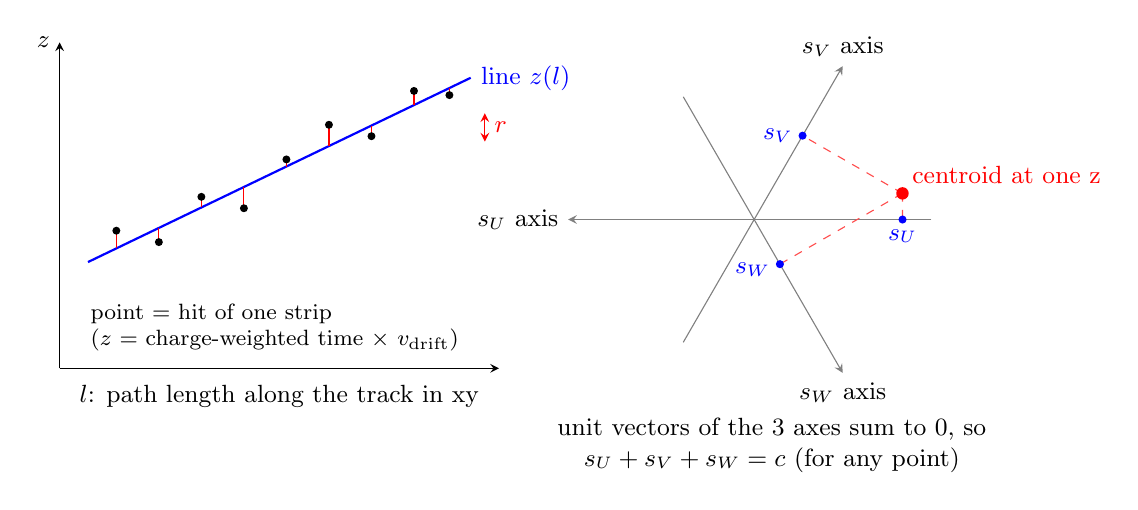
\begin{tikzpicture}[scale=0.9,>=stealth]
% left: z residual
\begin{scope}
\draw[->] (0,0) -- (6.2,0);
\node[font=\small] at (3.1,-0.4) {$l$: path length along the track in xy};
\draw[->] (0,0) -- (0,4.6) node[left,font=\small] {$z$};
\draw[thick,blue] (0.4,1.5) -- (5.8,4.1) node[right,font=\small] {line $z(l)$};
\foreach \x/\d in {0.8/0.25,1.4/-0.2,2.0/0.15,2.6/-0.3,3.2/0.1,3.8/0.3,4.4/-0.15,5.0/0.2,5.5/-0.1} {
  \pgfmathsetmacro{\zl}{1.5+(\x-0.4)*2.6/5.4}
  \draw[red,thin] (\x,\zl) -- (\x,\zl+\d);
  \fill[black] (\x,\zl+\d) circle (1.6pt);
}
\draw[<->,red] (6.0,3.2) -- (6.0,3.6);
\node[red,font=\small,right] at (6.0,3.4) {$r$};
\node[font=\footnotesize,align=left,anchor=south west] at (0.3,0.1) {point = hit of one strip\\($z$ = charge-weighted time $\times$ $v_\mathrm{drift}$)};
\end{scope}
% right: closure
\begin{scope}[xshift=9.8cm,yshift=2.1cm,scale=1.25]
\draw[->,gray] (180:-2.0) -- (180:2.1) node[left,font=\small,black] {$s_U$ axis};
\draw[->,gray] (60:-1.6) -- (60:2.0) node[above,font=\small,black] {$s_V$ axis};
\draw[->,gray] (-60:-1.6) -- (-60:2.0) node[below,font=\small,black] {$s_W$ axis};
\coordinate (P) at (10:1.7);
\coordinate (FU) at ($(180:-2)!(P)!(180:2)$);
\coordinate (FV) at ($(60:-2)!(P)!(60:2)$);
\coordinate (FW) at ($(-60:-2)!(P)!(-60:2)$);
\draw[dashed,red!70] (P) -- (FU); \draw[dashed,red!70] (P) -- (FV); \draw[dashed,red!70] (P) -- (FW);
\fill[blue] (FU) circle (1.3pt) node[below,font=\small,blue] {$s_U$};
\fill[blue] (FV) circle (1.3pt) node[left,font=\small,blue] {$s_V$};
\fill[blue] (FW) circle (1.3pt) node[left,font=\small,blue,yshift=-2pt] {$s_W$};
\fill[red] (P) circle (2pt) node[above right,font=\small,red] {centroid at one z};
\node[font=\small,align=center] at (0.2,-2.55) {unit vectors of the 3 axes sum to 0, so\\$s_U + s_V + s_W = c$ (for any point)};
\end{scope}
\end{tikzpicture}
\caption{The two residuals. Left: z residual = z of each hit minus the z predicted by the fitted line at the position of that hit.
Right: closure residual = deviation of the sum of the three view centroids at the same time from the geometric constant $c$ (no line used).}
\label{fig:resdef}
\end{figure}

\subsection{z residual (S11)}\label{sec:zres}
The robust $\sigma$ of the hit z residuals with respect to the line (Fig.~\ref{fig:resid}) is \textbf{0.19--0.22 mm $\approx$ 1 cell} at 232--502 ns (1 cell = 40 ns $\times$ 4.77 mm/\textmu s = 0.19 mm).
It is 0.25--0.31 mm at 1014 ns ($+30$--$60$\,\%) and 0.27 mm at 70 ns (insufficient S/N). It does not depend on the HV (GEMs 250 $\to$ 230 V, voltage sharing): 0.20--0.22.
Together with S12, \textbf{$\sigma_z$ is set by a distance, not by the timing} (candidate: strip width $\times$ track inclination $\approx 0.18$ mm).
The degradation at 1014 ns is the electronics timing precision added in quadrature ($\sqrt{0.31^2 - 0.21^2} \approx 0.23$ mm).
The RMS is 2--5 times the robust $\sigma$ (heavy tails), so fits must be robust.
Whether the pulse width can serve as the z error of a hit was an idea by S.~Aogaki tested here (it is not an established method); the answer is that it \textbf{overestimates the error by more than a factor of 10} (intrinsic width 14.5 cells = 2.8 mm, raw width 7--20 mm, measured 0.2 mm).

\begin{figure}[h]\centering
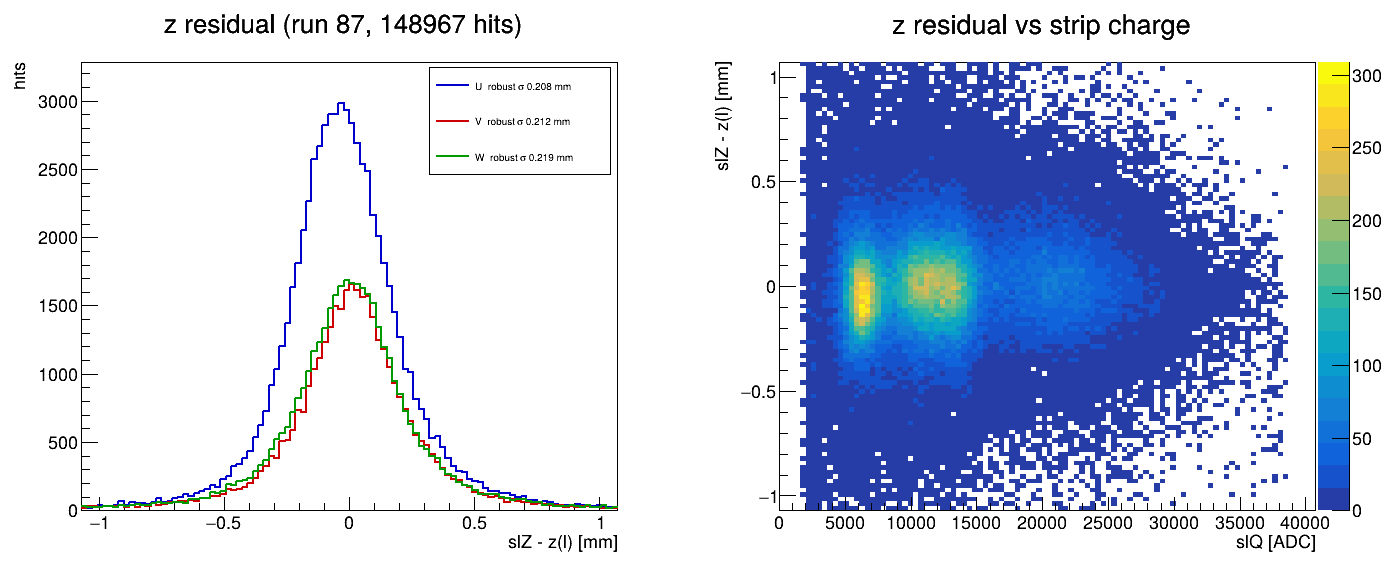
\includegraphics[width=0.95\textwidth]{fig/resid/run0087_resid.png}
\caption{S11: hit z residuals of run 87 (502 ns). Left: U/V/W, robust $\sigma$ 0.21--0.22 mm. Right: correlation with the strip charge.}
\label{fig:resid}
\end{figure}

\subsection{2D centroid precision = U/V/W closure residual (S14)}\label{sec:closure}
Definition in Sec.~\ref{sec:residual-def}, item 3. Only hit channels (strips that pass the condition of item 1) are used, and only their samples within $\pm 15$ cells of their own peak time (to remove late tails and halo). Only z slices where all three views form a single cluster are counted.
\textbf{The best value is 0.30 mm per view at 232 $\approx$ 502 ns}; 0.39--0.43 at 1014 ns (wide pulses spill out of the window) and 1.1 mm at 70 ns. No dependence on the GEM HV (0.30--0.32); slightly worse at 1,000 V drift (0.34).
The precision depends strongly on the charge (from 0.7--0.8 mm in the lowest to 0.40--0.45 mm in the highest charge quartile): the 2D precision is set by S/N.

Summary: at operating point B (502 ns) the error of a hit (z slab) is \textbf{$\sigma_s \approx 0.30$ mm (2D, per view) and $\sigma_z \approx 0.20$ mm}.

\begin{figure}[h]\centering
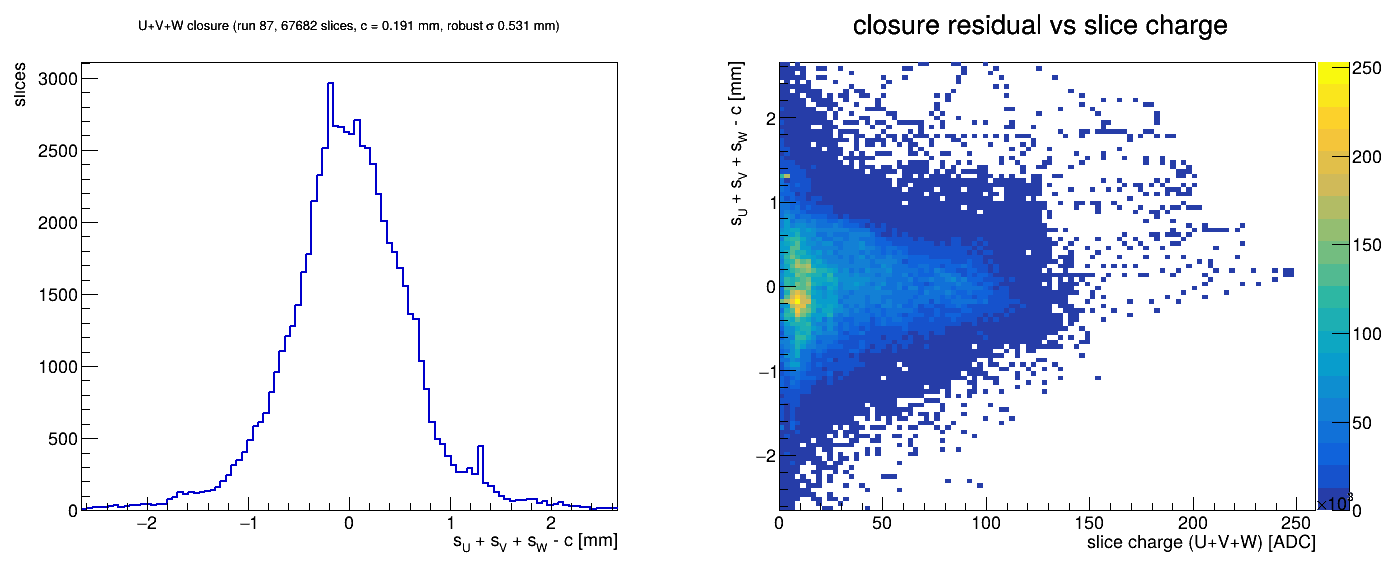
\includegraphics[width=0.95\textwidth]{fig/closure/run0087_closure.png}
\caption{S14: closure residual of run 87. Left: distribution, robust $\sigma$ 0.53 mm, i.e.\ $0.53/\sqrt{3} = 0.31$ mm per view. Right: correlation with the slice charge.}
\label{fig:closure}
\end{figure}

\section{Readout mode, rate and zero suppression}

\subsection{Readout and hit register (S9, S15)}
The partial readout used until then read all channels because the template had \texttt{channel Reading = always}; the hit-register threshold had no effect.
Moreover partial readout uses frameType 1 (4 B/sample), giving \textbf{twice} the data of full readout (frameType 2, 2 B/sample, 279 kB/event): 557 kB/event.
With a template using \texttt{Reading = only\_if\_hit} (S15) the threshold works (raising global / lsb goes from 400 to 241 kB), but because of the 4 B/sample it saves at most 14\,\% compared with full.
\textbf{Routine running therefore uses full readout}, and compression is left to ZS.

\subsection{Maximum rate (S17)}
The limits were measured with periodic triggers (no signal) and with the AsAd pulser ($-300$ mV on all 256 channels = 100\,\% occupancy).
\begin{itemize}
\item \textbf{The limit is the zCoBo FW readout time}: 2.94 ms for 272 channels ($\approx 340$ Hz with one AsAd), the same with full readout and with ZS. The event spacing is a constant ``period + 2.94 ms'', with no disturbance from network back-pressure.
\item \textbf{Triggers during readout are lost} (not queued): with a 2 ms pulser period every second pulse is recorded. Dead time = rate $\times$ readout time (29\,\% at 100 Hz with full readout).
\item \textbf{Readout time $\approx 0.11$ ms + 10.4\us $\times$ number of channels read}: with hit-partial readout and no signal (16 FPN channels) it is 0.28 ms (779 Hz). For an $\alpha$ event ($\approx 136$ channels) it is $\approx 1.5$ ms, i.e.\ 15\,\% at 100 Hz. \textbf{Hit-register partial readout is the only way to reduce the dead time.}
\item \textbf{ZS only reduces the bytes} (the readout time is unchanged): 65 kB even with all channels hit. Partial readout and ZS work together (frameType 1 + ZS).
\item 1 GbE has headroom up to 340 Hz with full readout (86 MB/s with a 1 ms pulser, at the edge). With partial readout and all channels hit (557 kB) it stops at 170 Hz. Fibre or 10 GbE does not help the zCoBo link (the FW Ethernet core is 1 GbE; see Sec.~\ref{sec:beam}).
\end{itemize}

\begin{table}[h]\centering\small
\caption{S17 maximum rate (runs 148--169).}
\footnotesize
\begin{tabular}{llrrrl}
\toprule
series & signal & rate [Hz] & min.\ spacing [ms] & kB/event & limit \\
\midrule
B full (272 ch) & none / pulser all ch & 254 / 310 & period + 2.94 & 279 & FW readout \\
hit partial g4 & none (16 FPN ch) & 779 & period + 0.28 & 33 & FW readout ($\propto$ ch) \\
hit partial g4 & pulser all ch (frameType 1) & 170 & 3.0 + stall & 557 & \textbf{1 GbE} \\
ZS per channel & pulser all ch & 333 & 3.0 & 65 & FW readout \\
hit partial + ZS & pulser all ch & 333 & 3.0 & 65 & FW readout \\
\bottomrule
\end{tabular}
\end{table}

\subsection{Zero suppression (S5, S13, S18)}
From a pedestal run (periodic trigger, full readout, 150 events) a per-channel table of mean and $\sigma$ was made (S5: median pedestal of the signal channels 456.5 ADC, median $\sigma$ 7.6--8.0, FPN $\sigma$ 3.3),
and threshold = pedestal $+ 5\sigma$ was put into the parameters as per-channel exceptions (\texttt{zs\_params.sh}).
ZS data contain no samples below threshold, so the usual algorithms that take the pedestal from the waveform (TPCReco's \texttt{PedestalCalculatorGRAW} as well as our macros) break.
On the DAQ side the same table is given as \texttt{[system] ped\_table} and used in three places: root\_sink (table mode of PEventTPC), the monitor (restoring the event display) and the analysis macros (\texttt{zs\_restore.C} fills the suppressed cells with the table values and writes a raw file of the same name, so the macros run unchanged).

The validation runs (S18, 1,500 events each, electronics of operating point B) are listed in Table~\ref{tab:zs}.
\textbf{ZS does not degrade the quality} (hit channels, ok, length, dEdx IQR, $\sigma_z$, $\sigma_{2D}$ equal to the reference; the total charge is $-3$\,\% from the sub-threshold tails).
Keeping the FPN channels improves no metric and costs $+32$ kB/event, so \textbf{the FPN channels are suppressed}.
The only processing ZS can affect in principle is waveform processing that uses the sub-threshold tails (deconvolution as in Sec.~2.2, or unfolding); hit, track and charge metrics are not affected.
Hit-partial g4 + ZS is the smallest (23.1 kB, 1/12) at the small price of $-4$ hit channels and $+12$\,\% in $\sigma_{2D}$. Since it is the only option that also reduces the dead time,
\textbf{the default candidate for beam runs is hit g4 + ZS (FPN suppressed)}; source runs use B full (current) or B + ZS.

\begin{table}[h]\centering\small
\caption{S18 ZS validation (runs 170--173, reference = run 130).}
\label{tab:zs}
\footnotesize
\begin{tabular}{rlrrrrrrr}
\toprule
run & setting & kB/event & hit ch & total charge & ok & length & $\sigma_z$ & $\sigma_{2D}$ \\
\midrule
130 & B full (reference) & 278.8 & 121.5 & 2.09 M & 0.998 & 84.4 & 0.21 & 0.314 \\
\textbf{170} & \textbf{B + ZS} & \textbf{30.9} (1/9) & 121 & 2.02 M & 0.998 & 83.9 & 0.20 & 0.320 \\
171 & B + ZS, FPN kept & 63.1 & 120 & 2.03 M & 0.997 & 83.2 & 0.20 & 0.319 \\
\textbf{172} & \textbf{hit g4 + ZS} & \textbf{23.1} (1/12) & 117 & 2.03 M & 0.996 & 82.9 & 0.19 & 0.357 \\
173 & hit g4 + ZS, FPN kept & 55.7 & 116 & 1.99 M & 0.997 & 82.0 & 0.19 & 0.354 \\
\bottomrule
\end{tabular}
\end{table}

\begin{figure}[h]\centering
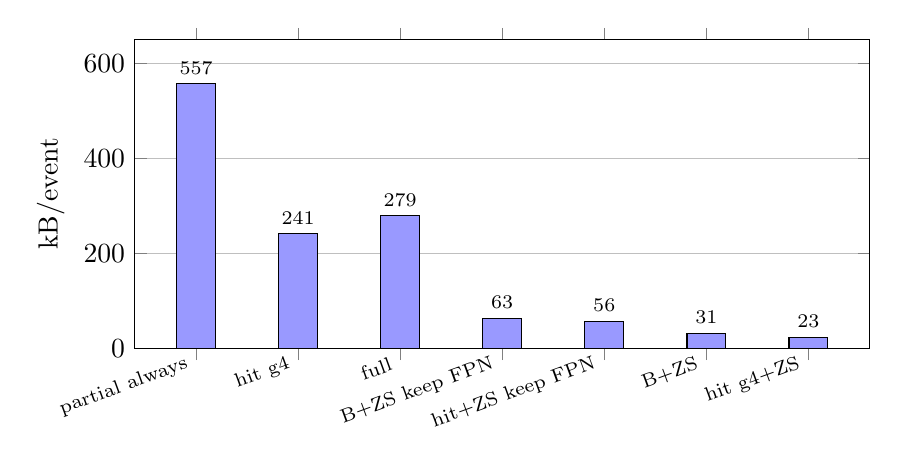
\begin{tikzpicture}
\begin{axis}[ybar,width=0.9\textwidth,height=5.5cm,ylabel={kB/event},symbolic x coords={partial always,hit g4,full,B+ZS keep FPN,hit+ZS keep FPN,B+ZS,hit g4+ZS},xtick=data,x tick label style={font=\scriptsize,rotate=20,anchor=east},nodes near coords,nodes near coords style={font=\scriptsize},ymin=0,ymax=650,bar width=14pt,ymajorgrids=true]
\addplot[fill=blue!40] coordinates {(partial always,557)(hit g4,241)(full,279)(B+ZS keep FPN,63)(hit+ZS keep FPN,56)(B+ZS,31)(hit g4+ZS,23)};
\end{axis}
\end{tikzpicture}
\caption{Data size per $\alpha$ event (S9, S15, S18).}
\end{figure}

\subsection{Design for beam runs ($\approx 100$ Hz)}\label{sec:beam}
The beam runs will not have a periodic trigger: \textbf{the particles arrive at random}, at an expected rate of $\approx 100$ Hz (more would be welcome). With random arrival the readout time $\tau$ acts as a non-paralysable dead time, and the accepted rate is $m = n/(1 + n\tau)$ (Table~\ref{tab:deadtime}).
Even at 100 Hz, full readout loses a quarter of the events, so hit-partial readout is worth more than with a periodic beam. The accepted rate saturates at $1/\tau$ (340 Hz full, $\approx 680$ Hz partial). With ZS the bandwidth, 23 kB $\times$ 300 Hz $\approx$ 7 MB/s, is no issue.

\begin{table}[h]\centering\small
\caption{Accepted rate for random arrival, $m = n/(1+n\tau)$.}
\label{tab:deadtime}
\begin{tabular}{rrr}
\toprule
true rate $n$ & full ($\tau$ = 2.94 ms) & hit partial ($\tau \approx 1.5$ ms, 136 ch as for $\alpha$) \\
\midrule
100 Hz & 77 Hz ($-23$\,\%) & 87 Hz ($-13$\,\%) \\
200 Hz & 127 Hz ($-37$\,\%) & 154 Hz ($-23$\,\%) \\
300 Hz & 160 Hz ($-47$\,\%) & 207 Hz ($-31$\,\%) \\
saturation & 340 Hz & $\approx 680$ Hz \\
\bottomrule
\end{tabular}
\end{table}

\textbf{The dead time must be measured.} The zCoBo does not assign an eventIdx to triggers that arrive during readout (only accepted triggers are numbered consecutively), so the number of lost triggers cannot be recovered from the data and the yields cannot be corrected. The raw external trigger pulses should be counted per run with a scaler (counting the zCoBo SMA OUT1, the latch pulse, in the same scaler gives the accepted number for comparison); on the DAQ side, $\tau$ can be estimated per run from ``0.11 ms + 10.4\us $\times$ channels read'' and logged.

\textbf{About 10 GbE.} Neither of the two zCoBo (ZC706) ports can run at 10 GbE. The RJ45 port uses the fixed MAC of the Zynq PS (at most 1 Gb/s; used at 100 Mbit for management by the FW). The SFP+ port is connected to a GTX transceiver that could run at 10 Gb/s in hardware, but the FW places a 1G AXI Ethernet core (1000BASE-X, line rate 1.25 Gb/s) in the PL and sends the data with the TCP stack of Linux on the ARM (checked in the boot log and README of the FW package). Optical modules (1000BASE-SX/LX) therefore work just like the copper adapter, but the speed stays at 1 GbE; a 10G-only module does not make it 10G (a module without 1G support will not link).
Going to 10G would require a new FW (a licensed 10G IP plus a TCP/UDP engine in the PL), and the 2.94 ms readout time would limit first anyway. This 2.94 ms is about twice what the AGET specification implies (512 cells $\times$ 68 channels at a 25 MHz readout clock $\approx 1.4$ ms per AGET), so there may be room in the readout part of the FW. \textbf{Question for the Warsaw group: which AGET readout clock does the zCoBo FW use?}

Estimate for ELITPC (Warsaw, two zCoBo $\times$ two AsAd): 544 channels per board $\to$ readout $\approx 5.8$ ms $\to$ saturation at 170 Hz with full readout and $-37$\,\% at 100 Hz random. With partial readout (25\,\% occupancy, $\approx 150$ channels) $\approx 1.7$ ms, i.e.\ $-15$\,\%.
The bandwidth is at the edge of 1 GbE (95 MB/s) with full readout and comfortable with partial + ZS. \textbf{Design for 100 Hz beam: hit-register partial readout + ZS + one 1 GbE link per board (merged into 10 GbE on the PC) + a trigger scaler.} Whether the FW readout time really doubles with two AsAd has to be measured in Warsaw.
Note: ZS graw files break the pedestal calculation of the offline grawToEventTPC. If ZS is used in Warsaw, we need to agree either to analyse our PEventTPC output (pedestal already subtracted with the table) or to add a pedestal-table input to TPCReco.

\section{Open issues and next steps}\label{sec:open}
\begin{itemize}
\item \textbf{Drift end (S6)}: even at 12.5 MHz with a 41\us window, the $\alpha$ tracks lie within 2--4\us of the trigger (Fig.~\ref{fig:drift}). The source is currently outside the chamber (attached to the gas line), and for solid-angle reasons the tracks barely extend in z, so tracks reaching the cathode side (20 cm) cannot be obtained in this configuration. The absolute $v_\mathrm{drift} = L / t_\mathrm{max}$ will be measured once the source is back inside the chamber. The bump near cell 340 does not move with the window position and is not physical (not understood).
\item \textbf{Source of the gas impurities}: whether the flow-dependent term $S$ (S19) comes from leaks or from outgassing is not yet separated. Humidity also matters (water permeation through tubing and O-rings scales with the room humidity; water absorbed in PCBs, Kapton and GEM foils is released; air entering through leaks carries water). \textbf{The dew point of the chamber gas is already measured, and it is the direct indicator}: the water partial pressure is fixed by the dew point, and around $-40\,^\circ$C a rise of 5--6 K means twice the water. If the doubling of $S/Q$ from 100 to 50 ml/min is due to water, the dew point must have risen by a few K at that time; if it did not move, the cause is something else (e.g.\ O$_2$ from a leak). To be checked by putting the dew-point record at the flow changes (16 Oct 12:08, 19 Oct 10:38) next to the charge trend (Fig.~\ref{fig:gas}). Converting to ppm needs the total pressure at the sensor, and if water from the bottle dominates the change will be small. An environment sensor (room temperature, humidity, pressure) and, once the source is inside, charge versus drift time will also help.
\item \textbf{Wiggle}: the 1.6--1.8\us component on $\alpha$ waveforms (signal channels only, proportional to the charge) is absent from the AGET response kernel; it may originate on the detector side (GEM / induction).
\item \textbf{Multiple tracks}: the present reconstruction fits one straight line per event. This is also behind the larger residual RMS at 502 ns than at 1014 ns (different outlier behaviour).
\item \textbf{Per-run ZS counters}: the ZS counters of root\_sink and the monitor are to be written into the run-stop record; the PEventTPC charge sum has not been cross-checked yet.
\end{itemize}

\begin{figure}[h]\centering
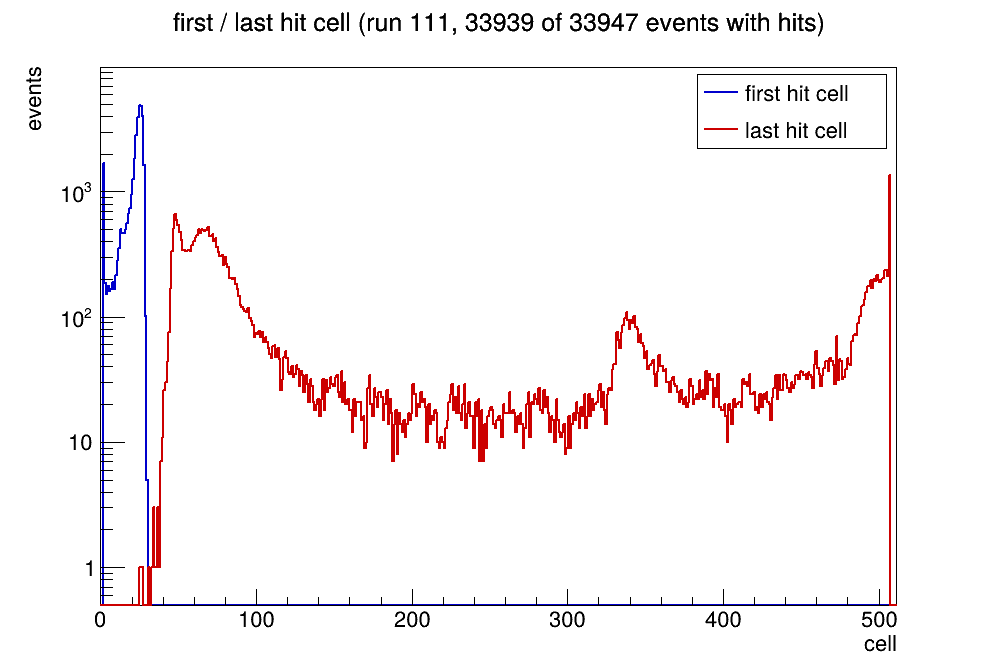
\includegraphics[width=0.6\textwidth]{fig/drift/run0111_drift.png}
\caption{S6: first / last hit cell of run 111 (12.5 MHz, delay 3800). The last hits cluster at 50--100 cells (2--4\us after the trigger); the spike at cell 508 is a window-edge artefact.}
\label{fig:drift}
\end{figure}

\FloatBarrier
\appendix
\section{Tools and records}
\begin{itemize}
\item Repository: \url{https://github.com/aogaki/tpcdaq-rs}. The DAQ source (Rust + C++), the specification, the operating procedures, the scan ledger and the tickets (design history and results) are all there. The developer documents are in Japanese. \textbf{English LLM translations of the documents listed below are in \path{docs/en/}} (index: \path{docs/en/README.md}); the Japanese originals are authoritative. For any other document, ask S.~Aogaki and an LLM translation will be prepared.
\item Scan ledger: \texttt{docs/SCANS\_ja.md} (S1--S19, the reference for all numbers; English: \path{docs/en/SCANS_en.md}). History and decisions: \texttt{TODO/archive/135--161} (English: \path{docs/en/tickets/}).
\item Tools: \path{tools/scan/} (\sloppy \texttt{scan.py}, \texttt{run\_metrics.C}, \texttt{metrics\_for\_run.sh}, \texttt{pulser\_kernel.C}, \texttt{deconv.C}, \texttt{drift\_end.C}, \texttt{hit\_residuals.C}, \texttt{uvw\_closure.C}, \texttt{gas\_trend.C}, \texttt{zs\_exceptions.py}, \texttt{zs\_params.sh}, \texttt{zs\_restore.C}, \texttt{ledger.py}); every macro has tests.
\item Specification: \texttt{docs/SPEC\_ja.md} v1.49 (ZS table mode, display restoration, ped\_table, decoder counters; English: \path{docs/en/SPEC_en.md}). Operation: \texttt{docs/RUNBOOK\_ja.md}, section on ZS operation (English: \path{docs/en/RUNBOOK_en.md}).
\end{itemize}

\section{Parameters of operating point B}
\texttt{base\_1750.json}. Knobs: \texttt{writingClockFrequency\_MHz} 25, \texttt{triggerDelay} 1750, \texttt{triggerMode} external, \texttt{peakingTime\_ns} 502, \texttt{gain} 120 fC, \texttt{readout} full, \texttt{fpnRead} true, \texttt{zeroSuppression.enabled} false.
Beam candidate: template \texttt{configure-elinp-hit.xcfg} (\texttt{channel Reading only\_if\_hit}), global 4 / lsb 15, ZS on with exceptions from \texttt{pedestal\_502ns.json} (FPN threshold 4095).
\end{document}
